\chapter{Evaluation} 
\label{chap:experiments}
Unless otherwise specified, the following experiments were conducted on a Dell Studio XPS Desktop, with 24 GB of RAM, and 8 Intel Core i-7 CPU X 980's @ 3.33GHz. The machine is running either 32-bit or 64-bit Ubuntu with the modified 3.10.9 Linux Kernel.

\section{Hrtimer Accuracy}
\label{sec:hrtimer}
The effectiveness of TimeKeeper's ability to keep virtual clocks synchronized is highly dependent on the $hrtimer's$ ability to fire interrupts at precise moments in time. For example, if we need a particular LXC to run for 1$\mu s$ at a time, then we would want the $hrtimer$ associated with that particular LXC to trigger an interrupt as close to 1$\mu s$ as possible. For the initial test, we set different $hrtimers$ to periodically fire at different time intervals ($timeslice$), and measured what time the $hrtimer$ interrupt actually fired. We collected 200 data points for every different time interval. From there, we calculated the mean ($\mu$) and standard deviation ($\sigma$) of the error. Table \ref{table:hrtimerAccuracy} presents the results.

\begin{table}\centering 
\begin{tabular}{|c|c|c|c|} 
        \hline 
        timeslice & $\mu$ & $\sigma$ \\ \hline 
        300$ms$ & 862ns &  1130ns \\ \hline 
        30$ms$ & 401ns &  680ns \\ \hline 
        3$ms$ & 341ns&  592ns \\ \hline 
        300$\mu s$ & 523ns &  2306ns \\ \hline 
        30$\mu s$ & 351ns &  2128 ns\\ \hline 
        3$\mu s$ & 481ns &  3312ns \\ \hline 
        1$\mu s$ & 2404ns &  4213ns \\ \hline 
        300$ns$ & 2925ns  & 6012ns \\ \hline 
        \hline 
        \end{tabular} 
        \caption{Mean and Standard Deviation of Timer Error for Different Timeslice Lengths} 
        \label{table:hrtimerAccuracy} 
\end{table}

Taking the first row as an example, when the timer was scheduled to fire an interrupt every 300$ms$, on average the interrupt occurred 862$ns$ from what was expected.  This is excellent accuracy, there are five orders of magnitude between the error and the $timeslice$. The magnitude of the variation in error is roughly constant; the error size relative to $timeslice$ is still an order of magnitude smaller with a 30 micro-second $timeslice$, and is roughly equal with a 3 micro-second $timeslice$.  These comparisons tell us something very important about the level of granularity we can effectively use in combined emulation/simulation scenarios.  If 10\% error in timing is acceptable and a simulated message takes on the order of 100 micro-seconds to pass on the network from one device to 
another, we can expect to get a little over three $timeslices$ in during the message's passage 
through the network simulator. {\em This} means that if a container is sensitive to IO from the simulator only at $timeslice$ boundaries (as is the case with the virtual-time OpenVZ system), there may be as much as a 33\% error in the virtual time at which the container ``sees" the message.    The take-away message here is that Linux timers are very accurate, but if we are to be able to take advantage of that accuracy when interfacing emulated LXC containers and a network simulator we will have to find a way to integrate simulator time and container time at a finer granularity than the $timeslice$.  This constitutes one of our areas of future work.

\section{Synchronization}
To integrate our emulation with network simulation we will need to keep LXCs closely synchronized.  We performed a set of experiments to evaluate how tightly we are able to do so. 
\subsection{Synchronized Experiment Accuracy}
In these experiments, TimeKeeper aimed to have each LXC achieve a target virtual time by the end of each $timeslice$. For each LXC and each $timeslice$ we measure the deviation of the virtual time the LXC actually achieved at that $timeslice$ from the target goal.  For each set of experiments we compute the mean error $\mu$ and the the standard deviation of the error $\sigma$, taken over all LXCs and synchronizations, and observe the behavior of these errors as a function of the number of LXCs and the size of the $timeslice$.  Our first round of experiments used the same TDF for all containers; 
each container was engaged in the compute-intensive task of computing the factorial of a large number.

\begin{table}\centering 
\begin{tabular}{|c|c|c|c|c|} 
        \hline 
       \# of LXCs & timeslice & $\mu$ & $\sigma$ \\ \hline 
        10 & .3ms & 596ns & 1084ns \\ \hline 
        10 & 3ms & 685ns & 1129ns \\ \hline 
        10 & 30ms & 1028ns & 1766ns \\ \hline 
        10 & 300ms & 812ns & 1447ns \\ \hline 
        80 & .3ms & 196ns & 375ns \\ \hline 
        80 & 3ms & 193ns & 374ns \\ \hline 
        80 & 30ms & 258ns & 535ns \\ \hline 
        80 & 300ms & 333ns & 628ns \\ \hline 
        \hline 
        \end{tabular} 
        \caption{Mean and Standard Deviation of Error as a Function of Timeslice and \#LXCs} 
        \label{table:msesamedil} 
\end{table}

For the first experiment, we used a TDF of 10 for each container, and recorded measurements for 150 $timeslice$ intervals. The results are summarized in Table \ref{table:msesamedil}, and reveal some interesting information. First, it demonstrates that TimeKeeper is effective at keeping virtual times synchronized on the $timeslice$ sizes used. TimeKeeper is seemingly more effective at keeping the experiment synchronized when the $timeslice$ length is 3$ms$ rather than 300$ms$. At the time of this writing we are unsure of the underlying cause for this difference, and are working at additional 
instrumentation in an effort to uncover an understandable explanation.

\begin{figure} \centering  
      \includegraphics[width=0.8\textwidth]{images/cdf_3ms_xnodes.eps} 
    \caption{CDF with timeslice=3ms as a function of \#LXCs} 
    \label{fig:sync1} 
  \end{figure} 

\begin{figure} \centering 
      \includegraphics[width=0.8\textwidth]{images/cdf_xms_10nodes.eps} 
    \caption{CDF with 10 LXCs as a function of timeslice length} 
    \label{fig:sync2} 
  \end{figure}

To give better insight into the distribution of error, we also plotted two cumulative distribution functions (CDFs). Figure \ref{fig:sync1} shows us a CDF when the number of LXCs in the experiment range from 10-80, and the $timeslice$ interval is constant at 3$ms$. Regardless of whether the experiment had 10 LXCs or 80 LXCs, TimeKeeper was able to keep every LXCs virtual time within 4$\mu s$ of the expected virtual time for more than 90\% of each $timeslice$ interval. However, this comes at a cost. The more LXCs you add to the experiment, the longer it takes for the experiment virtual time to progress. This will be explored more fully in Section \ref{sec:over}. Figure \ref{fig:sync2} shows us a CDF when we have an experiment size of 10 LXCs (where 5 LXCs have a TDF of 10, and 5 LXCs have a TDF of 1), and we vary the $timeslice$ interval lengths. In general, TimeKeeper is able to keep the experiment virtual time in sync, but we noticed when the $timeslice$ interval is .3$ms$ that it did not perform as well. These results correspond with what we found in Table \ref{table:hrtimerAccuracy} (where the $hrtimers$ were not as accurate at a granularity of .3$ms$ as opposed to higher granularities).

\subsection{Scalability}

Figure \ref{fig:scale} demonstrates scalability, plotting how the mean and standard deviation of the error behaves as the number of containers grows.  Again we see the interesting phenomena that the error decreases with increasing numbers of containers;  the error is also contained almost always to be less than half a micro-second. 

\begin{figure} \centering
      \includegraphics[width=0.8\textwidth]{images/scale.eps} 
    \caption{Testing Scalability with a Timeslice of 3ms and a TDF of 1/10} 
    \label{fig:scale} 
  \end{figure} 

We obtained access to a larger machine, with 32 cores and 64Gb of memory. This allowed us to stress test TimeKeeper and observe how many containers we can sustain.  We successfully did one experiment using 45,000 containers, which represents two orders magnitude increase of what could be done on that same machine with openVZ containers. 

We performed an experiment aimed at measuring the mean and standard deviation of the time error found when TimeKeeper tries to keep all LXC containers in an experiment synchronized. For this we keep the product of number of containers with the TDF constant, at approximately 20. The intuition is we are trying to keep the rate (in wallclock time) at which virtual time advances in the system as a whole constant---increasing the number of containers means the number of times a container is given service per unit wallclock time decreases, so each time it gets service it has to advance simulation time farther. Now in these experiments the $timeslice$ length is kept constant. 

\begin{figure} \centering 
      \includegraphics[width=0.8\textwidth]{images/mean_dev_large.eps} 
    \caption{Testing Scalability with the Product of \#LXCs and TDF Constant } 
    \label{fig:lxc_tdf_constant} 
  \end{figure} 

Figure \ref{fig:lxc_tdf_constant} displays the results, and reveals an interesting consequence of the scaling we employ. As the number of LXCs increases, the TDF decreases, which means that the advance in virtual time per unit wall-clock tick increases.  The error of timers {\em in wall-clock time} is unaffected by the number of containers, however this fixed error is {\em amplified} by the amplification of virtual time advancement.  This explains the linear increase in error.  We'd get essentially the same curve---but with different y-axis values---by using a different constant product of TDF and \#LXCs.  A product that is larger by a factor of 10 will yield errors that are a factor of 10 smaller.   Two main points should be appreciated from this data. One, that TimeKeeper has managed as many as 45,000 synchronized containers on a commodity server, and second, that the error of timers in real-time has more impact on the errors in virtual time the faster the containers are accelerated through virtual time.

\subsection{CS Accuracy}
In order to support CS, TimeKeeper needs to advance an LXC's virtual time by the amount specified by the user. Here, we explore how accurate TimeKeeper is at allowing a particular LXC to run to a specific period of time, then ensure it holds true when we scale the experiment to thousands of LXCs. For the experiment, we specified how long each LXC should be able to run by a static interval. Then we progressed each LXC by that interval, and calculated how far away the LXC's virtual time was from the expected virtual time. We collected 100 data points for each experiment, and modified either the interval in which the LXC's virtual time should advance at, or the number of LXCs in the experiment. The results can be found in Table \ref{table:cs_accuracy}.
\begin{table}\centering 
\begin{tabular}{|c|c|c|c|c|} 
        \hline 
       \# of LXCs & 10$\mu s$ & 100$\mu s$  & 1000$\mu s$  \\ \hline 
        8 & 2.05$\mu s$ & 9.79$\mu s$ & 67.2$\mu s$ \\ \hline 
        80 & 1.45$\mu s$ & 11.7$\mu s$ & 66.3$\mu s$ \\ \hline 
        800 & 1.88$\mu s$ & 12.13$\mu s$ & 63.5$\mu s$ \\ \hline 
        8000 & 2.0$\mu s$ & 9.34$\mu s$ & 66.9$\mu s$ \\ \hline 
        \hline 
        \end{tabular} 
        \caption{Average Error as a Function of the Virtual Time Advancement Interval and Number of LXCs} 
        \label{table:cs_accuracy}
\end{table}
The table suggests TimeKeeper is efficient at accurately maintaining the virtual times of LXCs via the CS method, regardless of the size of the experiment. With a 10$\mu s$ advancement interval, TimeKeeper was able to keep the error to within about 2$\mu s$. Another noticeable pattern is TimeKeeper appears to become more accurate as the advancement interval gets smaller. However, when the advancement interval gets too small, TimeKeeper actually becomes less accurate. This supports what we found in Section \ref{sec:hrtimer}. For example, when the advancement interval was 1$\mu s$, the average error was 6.24$\mu s$! 

\section{Overhead}
\label{sec:over}
For overhead experiments, we looked at two main areas. First, we look at how modifications to the kernel code affected the running time of the corresponding system calls. Next, we look at the overhead TimeKeeper introduces when it attempts to keep container's virtual times synchronized.
\subsection{Gettimeofday() Overhead}
The $gettimeofday()$ system call was the most heavily modified piece of kernel code, so we wanted to determine the level of impact these modifications have with respect to execution time. To test this, we created a process that would repeatedly call the $gettimeofday()$ system call with the normal Linux Kernel, measure how long each call would take, and calculate the average. Only the time spent executing the Kernel code was measured, the time spent switching from user-space to kernel-space was not measured.The experiment was repeated, but on our modified Linux kernel, and with TDF's of 1, .5, and 2. The results are summarized in Table \ref{table:gtodOverhead}.

\begin{table} \centering 
\begin{tabular}{|c|c|c|c|c|} 
        \hline 
         & Time ($ns$) & Difference ($ns$) & \% Longer \\ \hline 
        Unmodified Linux Kernel & 85.9 & 0 &  0 \\ \hline 
        Modified Linux Kernel, TDF 1 &  88.2 & 2.3 & 3 \\ \hline 
        Modified Linux Kernel, TDF .5 & 134.8 & 48.9 & 57 \\ \hline 
        Modified Linux Kernel, TDF 2 & 139.4 &  53.5 & 62 \\ \hline 
        \hline 
        \end{tabular} 
        \caption{Gettimeofday() Overhead} 
        \label{table:gtodOverhead} 
\end{table}

As you can see, the time difference between the unmodified Linux kernel $gettimeofday()$ system call and the modified Linux kernel $gettimeofday()$ system call is very small at 2.3$ns$. A majority of the processes on the system will not have a TDF, so this very small difference is good. When the process does have a TDF, the $gettimeofday()$ system call takes longer due to the additional complex operation of either multiplying or dividing two long numbers. However, this overhead is acceptable as a vast majority of the processes in any given system will by default not have TDFs. In addition, you notice the $gettimeofday()$ system call takes longer when the process has a TDF of 2, rather than .5. This is because a TDF $>$ 1 results in a division operation, which takes longer than the multiplication operation that occurs when the TDF $<$ 1.
\subsection{Gettimeofday() Overhead with vDSO Disabled}
\label{sec:expvdso}
As mentioned in Section \ref{subsec:vdso}, in 64-bit Linux it was necessary to modify parts of the vDSO in order for the modified $gettimeofday()$ system call to be executed. Here, we explore the additional overhead from making this modification. As in the previous experiment, we measured how long a single $gettimeofday()$ system call took to execute. This was repeated many times, and the average was calculated. This was tested on an unmodified Linux Kernel, as well as when the TDF was 1, 2, and .5. The results can be located in Table \ref{table:gtodvdso}.
\begin{table} \centering 
\begin{tabular}{|c|c|c|c|c|} 
        \hline 
         & Time ($ns$) & Difference ($ns$) & \% Longer \\ \hline 
        Unmodified Linux Kernel & 102 & 0 &  0 \\ \hline 
        Modified Linux Kernel, TDF 1 &  1248 & 1146 & 1123 \\ \hline 
        Modified Linux Kernel, TDF .5 & 1315 & 1213 & 1189 \\ \hline 
        Modified Linux Kernel, TDF 2 & 1380 &  1278 & 1253 \\ \hline 
        \hline 
        \end{tabular} 
        \caption{Gettimeofday() Overhead With vDSO Disabled} 
        \label{table:gtodvdso} 
\end{table}
As you can see, removing the $gettimeofday()$ system call from the vDSO caused a significant overhead increase. This makes sense, as when the vDSO is enabled, all the process needs to do is perform a few memory reads to determine the current time. It no longer needs to perform a context switch from user-space to kernel-space. With the vDSO disabled, our modified $gettimeofday()$ is actually called. Although this comes at the cost of additional overhead, we must remember it is in the granularity of $nanoseconds$. With that being said, the benefits brought by TimeKeeper outweigh the negative extra overhead.
\subsection{Synchronization Overhead}
We measured the scheduling overhead of TimeKeeper by dividing the amount of physical time progression of the leader LXC by the amount of time spent in the synchronization method of TimeKeeper. We call this the {\em overhead ratio} (OR). The larger the OR value, the more efficient the emulation. We ran multiple experiments with different TDFs and $timeslice$ lengths. We learned that as $timeslice$ length increases, so does the OR. This is intuitive, as a larger $timeslice$ will call TimeKeeper's synchronization function less frequently. 

Figure \ref{fig:overheadxn}(a) shows how the OR changes as the number of LXCs in an $experiment$ increases. For this particular experiment, the $timeslice$ was set to 3ms, and we scaled the number of LXCs from 10-160. As the number of LXCs grew, the OR decreased. This is because TimeKeeper must manage more LXCs, and managing these additional LXCs results in more overhead. This overhead can be reduced by dedicating more CPUs to the LXCs in the experiment. 

\begin{figure} \centering  
 \begin{tabular}{c} 
      \includegraphics[width=0.8\textwidth]{images/over_3ms_xn.eps} \\ 
      {\textbf{(a) 6 Dedicated CPUs and 24 GB RAM}}\label{subfig-1:over_small} \\ 
      \includegraphics[width=0.8\textwidth]{images/over_3ms_xn_large.eps} \\ 
      {\textbf{(b) 28 Dedicated CPUs and 64 GB RAM}}\label{subfig-2:over_large} 
  \end{tabular} 
    \caption{Overhead Ratio with Timeslice=3ms as a Function of \#LXCs} 
    \label{fig:overheadxn} 
  \end{figure} 

The overhead ratio calculated on a machine with 32 cores (28 dedicated cores) and 45,000 LXCs was {\bf .23} and is shown in Figure \ref{fig:overheadxn}(b). This is to be expected, and reducing that overhead will be explored in the following section.  
\subsection{Optimizing the Synchronization Overhead}
As we found previously, when the number of LXCs in an experiment was extremely large the amount of time spent in the synchronization phase dramatically increased. In fact, more time would be spent in the synchronization phase than time spent with allowing the LXCs time to advance! To reduce this overhead, we redesigned the synchronization phase to allow it to be run in parallel, with the work split up among a finite amount of threads. For the experiment, we compared the amount of time spent in the synchronization phase with our new optimized code verse the amount of time spent in the synchronization phase with the original code. We scaled the number of LXCs in the experiment and looked at the overall speedup. For the experiment, we allocated 8 threads for the synchronization phase, and the results can be found in Figure \ref{fig:sync_optimized}.
\begin{figure} \centering
      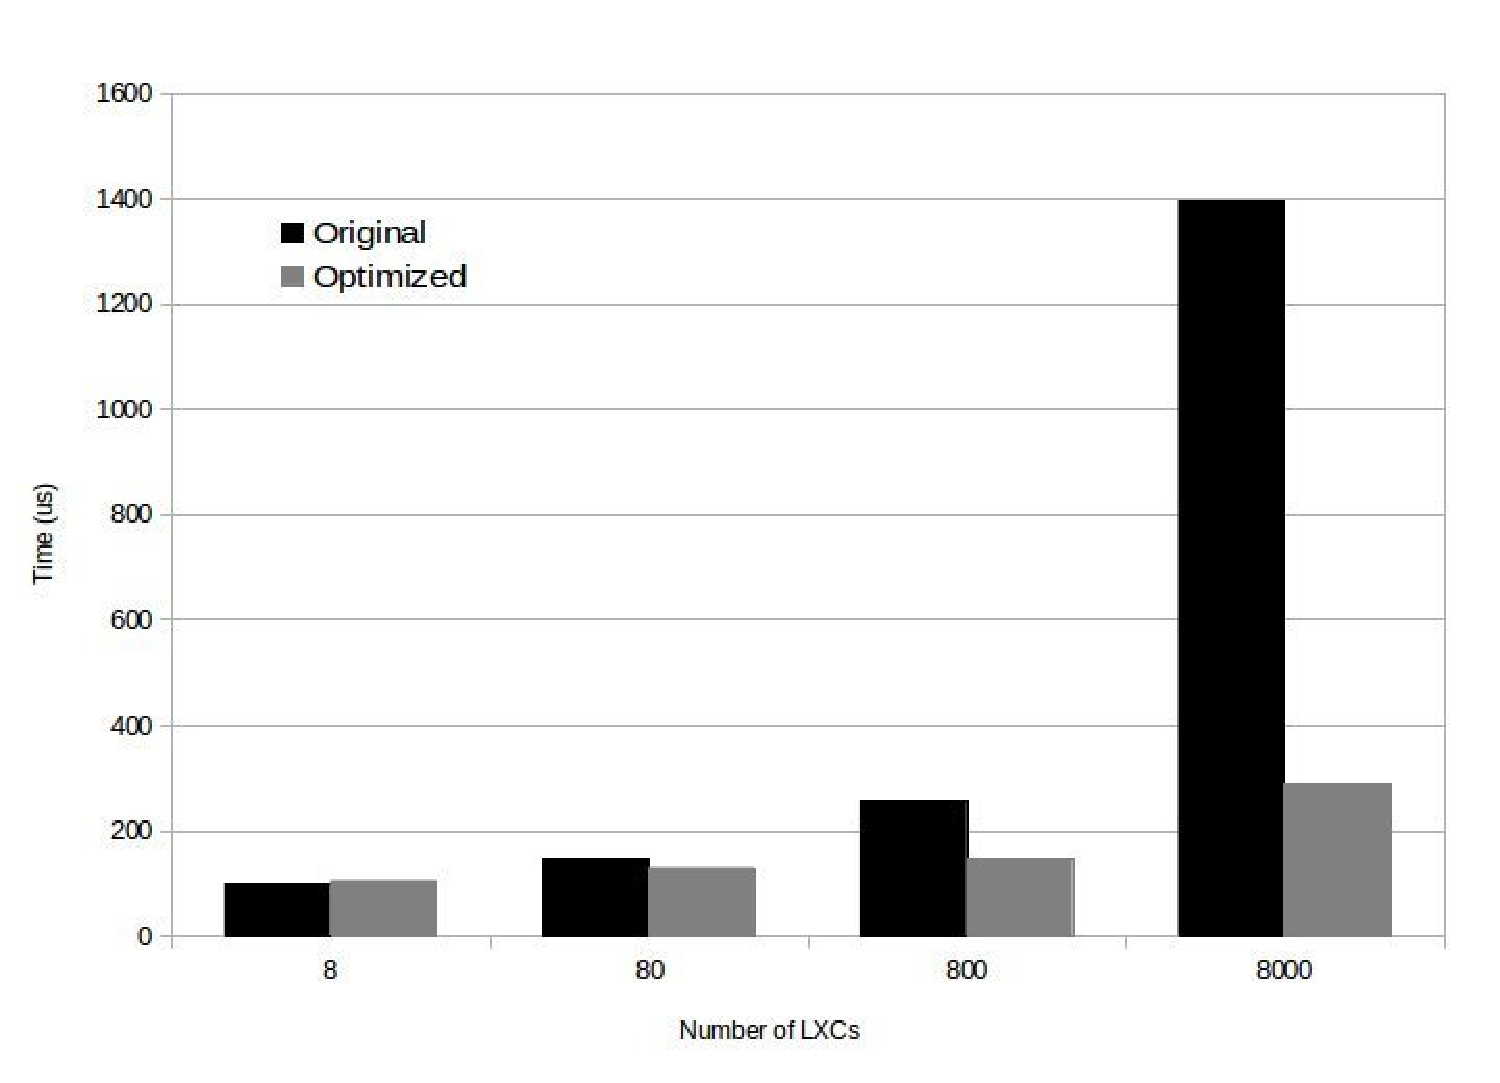
\includegraphics[width=0.8\textwidth]{images/sync_optimized.eps} 
    \caption{Time Spent in the Synchronization Phase} 
    \label{fig:sync_optimized} 
  \end{figure}  
Interestingly, when there are only 8 LXCs in the experiment, the optimized code is actually less efficient than the original code (with a speedup of .94x). This outcome is plausible, as needing to keep the 8 synchronization threads in parallel introduces some additional overhead. When the number of LXCs in the experiment is small, it is actually more efficient for one thread to go through each LXC and do the synchronization computation. However, a high improvement was seen when we ramped up the number of LXCs in the experiment to consist of 8000 LXCs. With 8000 LXCs, we found our optimized code to give us a 4.84x speedup as opposed to the original unoptimized code.
\section{Maintaining Real-Time}
We also wanted to determine how efficient TimeKeeper is at keeping LXCs running in real-time. When we say real-time, we mean that for every instant in time, all LXCs in the experiment will have a virtual time that is greater than or equal to the system time. Obviously, we will only be able to keep an experiment in real-time if all of its TDFs are all less than or equal to 1. For the experiment, we assumed all LXCs have the same TDF. Therefore, the maximum number of LXCs in an experiment we can keep in real-time is: N/TDF, where N is the number of dedicated CPUs on the machine, and we are assuming no overhead. However, our system does have overhead, so our experiment will determine just how close we can get to this upper bound. We ran experiments with 6 dedicated CPUs, a $timeslice$ of 3$ms$, and TDFs of 1/10, 1/50, and 1/100 with increasing numbers of LXCs per experiment, until we found the tipping point (the point where we could no longer keep the experiment as a whole in real- time). We calculated the virtual time of each LXC and compared it to the system time at the end of each $timeslice$ interval. Our results are in Figure \ref{fig:rt}. 

\begin{figure} \centering  
 \begin{tabular}{c} 
      \includegraphics[width=0.8\textwidth]{images/optimal.eps} \\ 
      {\textbf{(a) 6/(TDF+1) \#LXCs}}\label{subfig-1:rtopt} \\ 
      \includegraphics[width=0.8\textwidth]{images/notoptimal.eps} \\ 
      {\textbf{(b) 6/(TDF+1) +1 \#LXCs}}\label{subfig-2:rtnotopt} 
  \end{tabular} 
    \caption{Determining Maximum \#LXCs Where Real-Time is Maintained} 
    \label{fig:rt} 
  \end{figure} 
We found the maximum number of LXCs to be: $6/(TDF+1)$, any more LXCs cause a tipping point and the experiment can no longer be kept in  real-time. Figure \ref{fig:rt}(a) displays the virtual time of the experiment with respect to the system time using this tipping point. As you can see, all experiments virtual time is $increasing$ linearly in respect with the system time. Figure \ref{fig:rt}(b) displays the same thing, but this time, adding just 1 more LXC to each experiment, ie: $6/(TDF+1)+1$. This is obviously the tipping point, as all three experiments virtual time is now $decreasing$ with respect to the system time.
\section{CORE Experiments}
\label {sec:core_experiments}
Here we will discuss experiments conducted with TimeKeeper while it was fully integrated with CORE. 
\subsection{Verifying Network Bandwidth}
The following experiments consisted of basic network analysis with CORE while TimeKeeper is integrated. Within TimeKeeper's notion of a synchronized experiment, some containers may be frozen for large periods of time, allowing other container's time to 'catch up'. Consider the example when one container has a TDF of 10 and another has a TDF of 1. In this scenario, the container with a TDF of 1 will only be allowed to run 1/10 the time of the container with a TDF of 10. Therefore, it is important for the fidelity of the experiment that freezing/unfreezing a container does not interfere with the packet flow of the application. The experiment consisted of a simple 3-node topology, with one switch, one server, and one client. The $iperf$ tool was used to measure the bandwidth between the client and the server. The experiment was repeated numerous times, calculating the average bandwidth, CPU utilization, and experiment length. This process was collected across experiments with varying TDFs, and the results can be found in Figure \ref{fig:core_exp}.
\begin{figure} \centering
 \begin{tabular}{c} 
      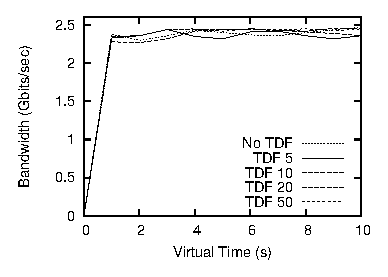
\includegraphics[width=0.8\textwidth]{images/core_iperf.eps} \\ 
      {\textbf{(a) 6/(TDF+1) \#LXCs}}\label{subfig-1:core_iperf} \\ 
      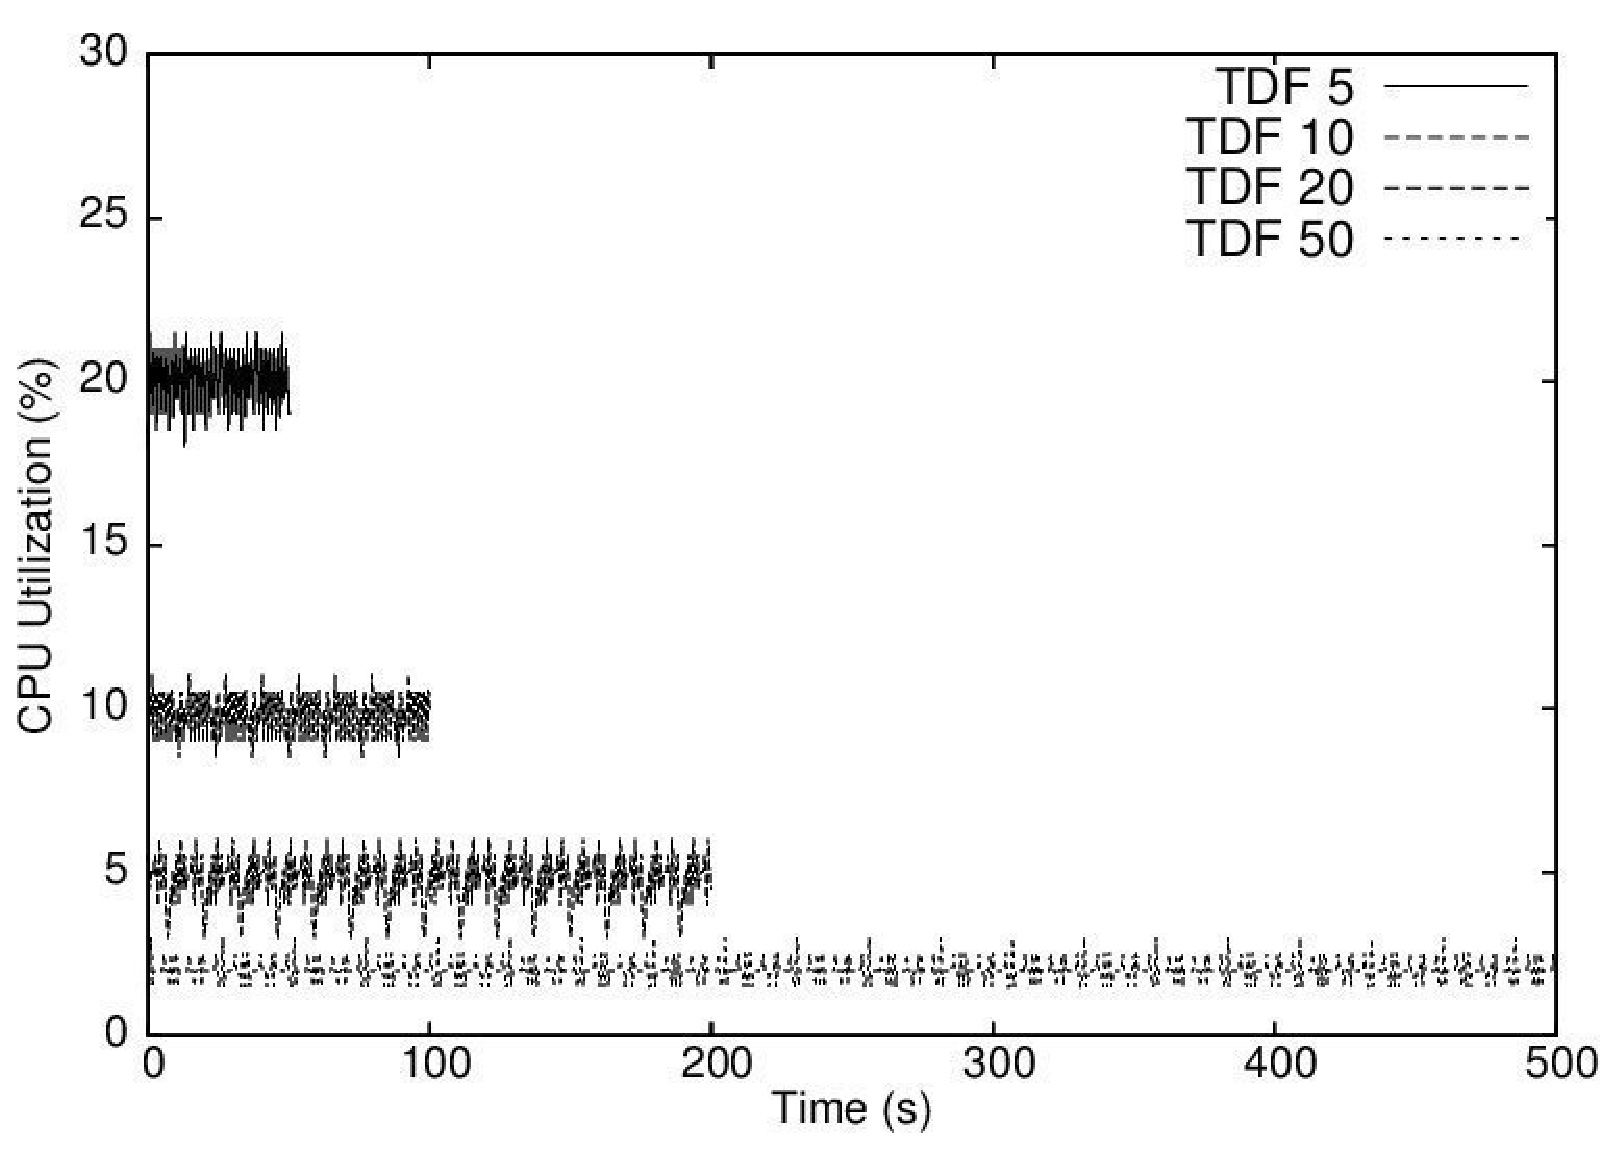
\includegraphics[width=0.8\textwidth]{images/core_cpu.eps} \\ 
      {\textbf{(b) 6/(TDF+1) +1 \#LXCs}}\label{subfig-2:core_cpu} 
  \end{tabular} 
    \caption{Determining Maximum \#LXCs Where Real-Time is Maintained} 
    \label{fig:core_exp} 
  \end{figure} 
Figure \ref{fig:core_exp}(a) displays the resulting bandwidth across time using different TDFs. As you can see, regardless of whether or not the experiment was running in real-time (the case where no TDF is used), or much slower than real-time (where the TDF is 50), the resultant bandwidth is approximately the same. This is very promising, and helps support our claim that a time-dilated experiment will return the same results as an experiment ran without a TDF. Next, Figure \ref{fig:core_exp}(b) explores how different TDFs have an effect on the CPU utilization, as well as the overall time necessary to run an experiment. When the experiment is conducted without a TDF, the $iperf$ process takes approximately 10 seconds to run, and demands 100\% of the CPU in order to send as many packets as possible. This default case is not shown in Figure \ref{fig:core_exp}(b) in order to show in more detail what is going on when the synchronized experiment is assigned a TDF. As the TDF of a synchronized experiment increases, the CPU utilization of the $iperf$ process is decreased with respect to the TDF. However, this comes at the cost of a longer overall experiment runtime. Figure \ref{fig:core_exp}(b) demonstrates that when the TDF of the experiment is 50, the $iperf$ process only spends approximately 2\% of its time on the CPU. However, the same experiment will now takes 500 seconds to run. This tradeoff between system utilization and experiment runtime is beneficial to an extent. A lower system utilization will allow us to run more complex topologies with a network simulator, and this is further explored in Section \ref{sec:ns3_experiments}. \\ 
The previous experiment demonstrated TimeKeeper's ability to maintain a consistent bandwidth with a simple 3-node topology. Here, the experiment was extended to be more complex. This time, an additional 100 containers were added to the experiment, and were configured to randomly send messages to one another. This increases the complexity in two ways. First, the number of containers TimeKeeper needs to synchronize is increased by a factor of 50. Next, additional background traffic is added, as the new containers randomly talk to one another. Once again, the experiment was ran with numerous different TDFs, and the average bandwidth as measured. Similar to the previous experiment, we found the bandwidth to be consistent across all runs. The additional containers did not affect TimeKeeper's ability to maintain a consistent bandwidth; however, it did increase the overall experiment runtime. The overall bandwidth was lower than the overall bandwidth in the previous experiment, but this makes sense as the additional background traffic is running concurrently with the $iperf$ process.
\section{NS-3 Experiments}
\label {sec:ns3_experiments}
Here we will discuss experiments ran with TimeKeeper integrated with ns-3. 
\subsection{Measuring Jitter with a Non-Overloaded Simulator}
In ns-3, $jitter$ is defined as the difference in time between when a event should be processed in the simulator and when the event actually is processed. When running ns-3 with the RealTime Scheduler, reducing the jitter is very important to increase the fidelity of the experiment. When the RealTime Scheduler is running in $Hard Limit$ mode, it will abruptly stop if the jitter gets above a certain point (the default is 100ms). The following experiments were developed to investigate how TimeKeeper may be utilized to reduce the overall jitter within a simulation. First, a simple ns-3 network was created which consisted of a server and a client (both the server and the client were LXCs). Both nodes communicated via the WiFi network model provided by ns-3. We performed an $iperf$ between the client and the server, measuring the jitter for every single event. This procedure was repeated across experiments with many different TDFs. The results are found in Figure \ref{fig:nonoverloaded}.
\begin{figure} \centering  
      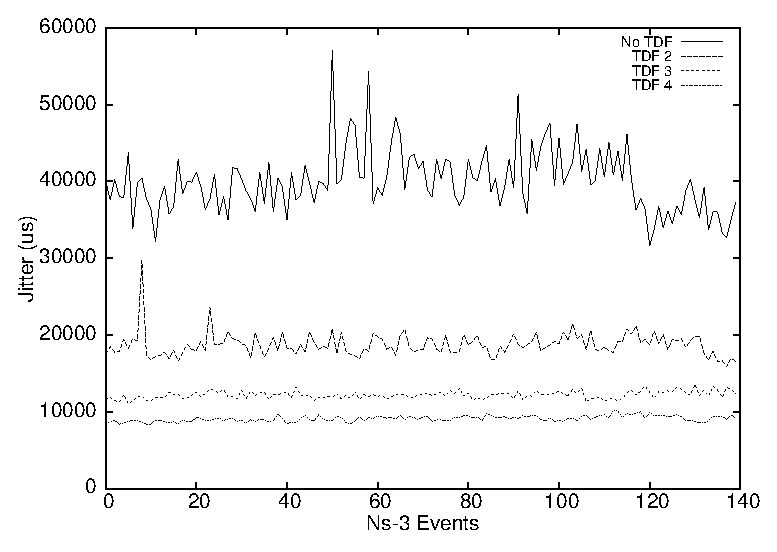
\includegraphics[width=0.8\textwidth]{images/jitter_nonoverloaded.eps} 
    \caption{Jitter Non-Overloaded WiFi Model} 
    \label{fig:nonoverloaded} 
  \end{figure}  
As you can see, the simulator was never overloaded, because for every single experiment the jitter was below the default $HardLimit$ of 100ms. The average jitter for a non time-dilated experiment was about 40ms. When the experiment was repeated with TDFs of 2, 3, and 4, the resulting average jitter was 18.7ms, 12.2ms, and 9.1ms respectively. The reduction in jitter was anticipated, as the TDF specifies how long an experiment should take to run, and the average jitter will be reduced by the factor of the TDF. \\
\subsection{Measuring Jitter with a Overloaded Simulator}
Next, we look at how the jitter is affected when the simulator was overloaded. From the previous CORE experiments (in Section \ref{sec:core_experiments} we learned that with a high TDF the synchronized experiment will progress through virtual time more slowly, thus reducing the stress on the simulator.  Therefore, a simulation which was previously overloaded should be able to complete and give accurate results if given a high enough TDF. To create an overloaded experiment, we constructed a simple ns-3 network using the CSMA network model. Once again, we had a client and a server, and the  client would perform an $iperf$ to measure the bandwidth. This situation originally overloads the simulator, because the CSMA network model attempts to provide higher bandwidth than the WiFi network model, and the additional packet events bog down the simulator. Once again, we recorded the jitter for every event, and repeated this procedure for experiments with different TDFs. The results are found in Figure \ref{fig:overloaded}.
\begin{figure} \centering  
      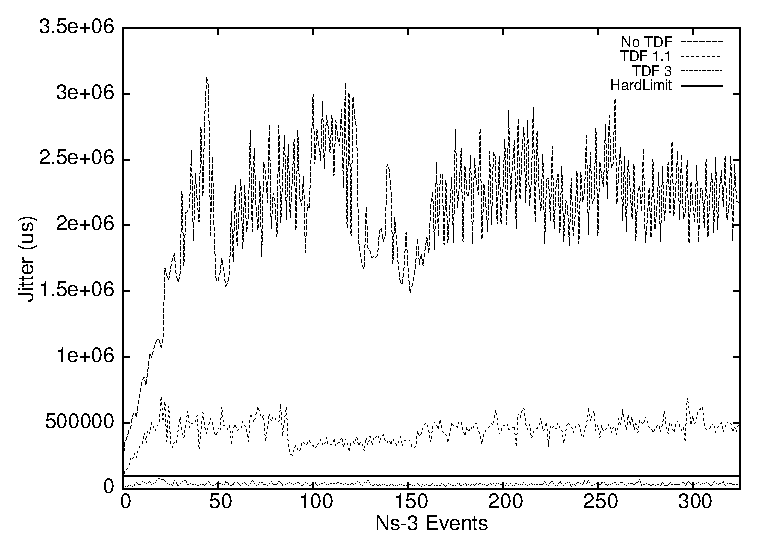
\includegraphics[width=0.8\textwidth]{images/jitter_overloaded.eps} 
    \caption{Jitter Overloaded CSMA Model} 
    \label{fig:overloaded} 
  \end{figure}
  When the simulator was overloaded, the average jitter is hurt dramatically. When the experiment did not have a TDF, the average jitter was 2108ms, or roughly 20x greater than the RealTime Scheduler's default $HardLimit$. An improvement is seen when the experiment is given a TDF of 1.1, which cuts the average jitter down to 441ms. Increasing the experiments TDF to 3 further reduces the average jitter down to 35.4ms. When the TDF is 3, it is considered a successful experiment, as the jitter never exceeds the default $HardLimit$. 
\subsection{Increasing Network Complexity}
While we have demonstrated that increasing the TDF of an experiment will reduce the average jitter in a simple experiment, we wanted to ensure the same held true in a more complicated network as well. This was done by constructing a network topology which consisted of 100 ns-3 nodes. These nodes would communicate with one another over the WiFi network model to provide background traffic, as well as cause extra stress on the ns-3 simulator. In addition, we tied in two LXCs who were connected to the same network model, and performed a $iperf$ test between them. This more complicated topology was able to overload the ns-3 simulator, unlike the previous WiFi network model example. We ran the experiment with various TDFs and calculated the average jitter. The results can be found in Table \ref{table:complexns3}.
\begin{table}\footnotesize\centering 
\begin{tabular}{|c|c|} 
        \hline 
        TDF & Runtime\\ \hline 
        None & 1700ms \\ \hline 
        2 & 738ms \\ \hline 
        3 & 312ms \\ \hline 
        4 &  101ms \\ \hline 
        5 & 30ms \\ \hline 
        10 & 4.25ms \\ \hline 
        \hline 
        \end{tabular} 
        \caption{Average Jitter with Large Ns-3 WiFi Model} 
        \label{table:complexns3} 
\end{table}
Similar to the previous experiment regarding jitter, as the TDF increased the average jitter decreased. When the TDF of the experiment was 5 or 10, the jitter remained under the default $Hard Limit$ of the RealTime Scheduler, and would be able to finish successfully and give accurate results. The size of the experiment did not seem to affect TimeKeeper's ability to reduce the average jitter. We were able to run more complicated experiments that would have previously failed out or given inaccurate results. This is done setting a high experiment TDF to reduce the average jitter; however, it is important to remember that this comes at the cost of higher experiment runtime.
\section{Current Limitations}
\label{sec:limitations}
In this section, we will discuss a comprehensive list of TimeKeeper's limitations. We will describe how these limitations do not prevent TimeKeeper from achieving its design goals. 
\subsection{Adequate Hardware}
TimeKeeper will be limited in its ability to function properly if the system in which it is installed on is relatively old. Here, relatively old is considered to be a system where it only has one or two vCPUs (even with hyperthreading), and less than 4 GB of RAM. This system would not be ideal for TimeKeeper, as the user needs to set specific vCPUs in which TimeKeeper will be allowed complete control. If there are only one or two such vCPUs, TimeKeeper will most likely overload the system, and normal background Linux tasks will not be able to complete. Therefore, it is imperative TimeKeeper is installed on a system with at least four vCPUs. We do not think this is an outrageous demand, as most standard laptops on the market currently start out with four vCPUs. 
\subsection{Manipulating LXCs Correctly}
There are two standard ways in which most people use LXCs. One method creates the LXC and starts a bash terminal. From here, the user can manually interact with this terminal by running various commands and scripts. TimeKeeper directly supports this method, and has no problems. The other method is to start the LXC as a daemon, and use the $lxc$-$attach$ tool to run specific commands from within the LXC. This is more common if you want to create many LXCs, and having so many open terminals would be extremely cumbersome. Here is where a problem arises with TimeKeeper. Recall TimeKeeper interacts with a LXC and all of the LXC's children via a linked list in the $task\_struct$. The process created from $lxc$-$attach$ is not actually a child of the LXC; rather, it is created externally and then pushed into the LXC's namespace. Therefore, TimeKeeper is not able to handle this new process correctly, as it is not technically a child of the LXC, and not found when TimeKeeper traverses the LXC's linked list of children. However, a workaround was developed to quickly and easily run commands from within LXC daemons, and the process is outlined in Figure \ref{fig:lxc_commands}. 
\begin{figure}[t] 
      \includegraphics[width=\textwidth]{images/lxc_commands.eps} 
    \caption{Running Commands From Within an LXC Daemon} 
    \label{fig:lxc_commands}
  \end{figure}
For example, lets use $lxc$-$1$ for the name of the LXC. We start the LXC as a daemon with the command $lxc$-$start\ $-$n\ lxc$-$1\ $-$d\ ./reader$. The $reader$ script will get executed when the daemon is started. All the $reader$ script will do is create a named pipe in the /tmp directory based on the name of the LXC, and wait for data to be sent to the named pipe. When data arrives, the $reader$ will try to execute whatever was sent, and store the output of the command in a data directory. So to have the LXC run the $ls$ command to print the files in the current directory, you simply need to run $echo\ ls\ >\ /tmp/lxc$-$1$. To see the output of running the command, simply read data/lxc-1. This method allows us to quickly spawn up many daemons and have them run commands simultaneously with TimeKeeper functioning properly.
\subsection{Kernel Crashes}
It is nearly impossible to claim a complex LKM to be completely bug free, and TimeKeeper is no exception. If the user runs TimeKeeper as it was intended, and uses the API functions in the correct order, TimeKeeper will rarely crash. However, there still exist some edge cases TimeKeeper does not correctly handle if things do not go as planned. In this case, TimeKeeper will most likely crash, and the computer will need to be restarted before TimeKeeper can be run correctly again. 
\subsection{Distributed TimeKeeper}
Currently, TimeKeeper only brings a notion of virtual time to one physical system. It is currently not possible to have two separate machines achieving virtual time synchronization simultaneously. Distributed TimeKeeper would be a great idea for future work. The ability to spread TimeKeeper out over multiple machines, or even a physical testbed, would allow for much larger experiments than previously possible.
